\hypertarget{motivauxe7uxe3o}{%
\section{Motiva\c{c}\~{a}o}\label{motivauxe7uxe3o}}

\begin{frame}{Limita\c{c}\~{o}es do Analisador Ad-Hoc}
\protect\hypertarget{limitauxe7uxf5es-do-analisador-ad-hoc}{}
\begin{itemize}
\tightlist
\item
  Difícil de manter e extender para linguagens maiores
\item
  Como adicionar \textbf{identificadores}? Exige reestruturar o estado
\end{itemize}
\end{frame}

\begin{frame}[fragile]{Limita\c{c}\~{o}es do Analisador Ad-Hoc}
\protect\hypertarget{limitauxe7uxf5es-do-analisador-ad-hoc-1}{}
\begin{itemize}
\tightlist
\item
  Como suportar \textbf{comentários em bloco}
  (\passthrough{\lstinline!/* */!})?
\item
  Como garantir que a implementa\c{c}\~{a}o está correta?
\end{itemize}
\end{frame}

\begin{frame}{Limita\c{c}\~{o}es do Analisador Ad-Hoc}
\protect\hypertarget{limitauxe7uxf5es-do-analisador-ad-hoc-2}{}
\begin{itemize}
\tightlist
\item
  Pergunta: existe uma forma extensível e eficiente para construir
  analisadores?
\end{itemize}
\end{frame}

\begin{frame}{A Solu\c{c}\~{a}o: Express\~{o}es Regulares + Aut\^{o}matos}
\protect\hypertarget{a-soluuxe7uxe3o-expressuxf5es-regulares-autuxf4matos}{}
\begin{itemize}
\tightlist
\item
  Especificamos tokens como \textbf{express\~{o}es regulares} (declarativo)
\item
  Geramos o analisador léxico \textbf{automaticamente} a partir dessa
  especifica\c{c}\~{a}o
\end{itemize}
\end{frame}

\begin{frame}{A Solu\c{c}\~{a}o: Express\~{o}es Regulares + Aut\^{o}matos}
\protect\hypertarget{a-soluuxe7uxe3o-expressuxf5es-regulares-autuxf4matos-1}{}
\begin{itemize}
\tightlist
\item
  O analisador gerado é um \textbf{Aut\^{o}mato Finito Determinístico (AFD)}
\item
  Garantias formais de corre\c{c}\~{a}o e efici\^{e}ncia
\item
  Teoria bem estabelecida: linguagens regulares
\end{itemize}
\end{frame}

\hypertarget{autuxf4matos-finitos-determinuxedsticos}{%
\section{Aut\^{o}matos Finitos
Determinísticos}\label{autuxf4matos-finitos-determinuxedsticos}}

\begin{frame}{Defini\c{c}\~{a}o Formal}
\protect\hypertarget{definiuxe7uxe3o-formal}{}
Um AFD \(M = (E, \Sigma, \delta, i, F)\):

\begin{itemize}
\tightlist
\item
  \(E\): conjunto finito de \textbf{estados}
\item
  \(\Sigma\): \textbf{alfabeto} de entrada
\item
  \(\delta : E \times \Sigma \to E\): \textbf{fun\c{c}\~{a}o de transi\c{c}\~{a}o}
  (determinística)
\item
  \(i \in E\): \textbf{estado inicial} único
\item
  \(F \subseteq E\): conjunto de \textbf{estados finais} (aceita\c{c}\~{a}o)
\end{itemize}
\end{frame}

\begin{frame}[fragile]{Representa\c{c}\~{a}o em Haskell}
\protect\hypertarget{representauxe7uxe3o-em-haskell}{}
\begin{lstlisting}[language=Haskell]
data DFA a = DFA
  { start  :: a           -- estado inicial
  , delta  :: a -> Char -> a  -- fun\c{c}\~{a}o de transi\c{c}\~{a}o
  , finals :: a -> Bool   -- predicado de estado final
  }
\end{lstlisting}

\begin{itemize}
\tightlist
\item
  Parametrizado pelo tipo \passthrough{\lstinline!a!} dos estados
\item
  A fun\c{c}\~{a}o \passthrough{\lstinline!finals!} retorna
  \passthrough{\lstinline!True!} para estados finais
\item
  Flexível: estados podem ser \passthrough{\lstinline!Bool!},
  \passthrough{\lstinline!Int!}, \passthrough{\lstinline!Set Int!}, etc.
\end{itemize}
\end{frame}

\begin{frame}[fragile]{Exemplo: AFD para Palavras Terminadas em
\passthrough{\lstinline!1!}}
\protect\hypertarget{exemplo-afd-para-palavras-terminadas-em-1}{}
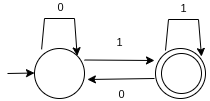
\includegraphics[width=0.6\textwidth,height=\textheight]{chapter03/imgs/afd.png}

\begin{itemize}
\tightlist
\item
  Estado \passthrough{\lstinline!False!}: último caractere n\~{a}o foi
  \passthrough{\lstinline!1!} (ou início)
\item
  Estado \passthrough{\lstinline!True!}: último caractere foi
  \passthrough{\lstinline!1!} (estado final)
\end{itemize}
\end{frame}

\begin{frame}[fragile]{Implementa\c{c}\~{a}o do AFD}
\protect\hypertarget{implementauxe7uxe3o-do-afd}{}
\begin{lstlisting}[language=Haskell]
endsWithOne :: DFA Bool
endsWithOne = DFA False transition id
  where
    transition False '0' = False
    transition False '1' = True
    transition True  '0' = False
    transition True  '1' = True
    transition _     _   = False
\end{lstlisting}

\begin{itemize}
\tightlist
\item
  Estado inicial: \passthrough{\lstinline!False!}
\item
  Fun\c{c}\~{a}o final: \passthrough{\lstinline!id!} (só
  \passthrough{\lstinline!True!} é estado final)
\item
  Transi\c{c}\~{o}es por casamento de padr\~{o}es
\end{itemize}
\end{frame}

\begin{frame}[fragile]{Execu\c{c}\~{a}o e Aceita\c{c}\~{a}o}
\protect\hypertarget{execuuxe7uxe3o-e-aceitauxe7uxe3o}{}
\begin{lstlisting}[language=Haskell]
-- Computa o estado final após processar toda a string
deltaStar :: DFA a -> String -> a
deltaStar m = foldl (delta m) (start m)

-- Verifica se uma string é aceita
accept :: DFA a -> String -> Bool
accept m s = finals m (deltaStar m s)
\end{lstlisting}

Exemplos:

\begin{itemize}
\tightlist
\item
  \passthrough{\lstinline!accept endsWithOne "01"!} →
  \passthrough{\lstinline!True!}
\item
  \passthrough{\lstinline!accept endsWithOne "10"!} →
  \passthrough{\lstinline!False!}
\item
  \passthrough{\lstinline!accept endsWithOne "001"!} →
  \passthrough{\lstinline!True!}
\end{itemize}
\end{frame}

\hypertarget{autuxf4matos-finitos-nuxe3o-determinuxedsticos}{%
\section{Aut\^{o}matos Finitos
N\~{a}o-Determinísticos}\label{autuxf4matos-finitos-nuxe3o-determinuxedsticos}}

\begin{frame}{Defini\c{c}\~{a}o Formal}
\protect\hypertarget{definiuxe7uxe3o-formal-1}{}
Um AFN \(M = (E, \Sigma, \delta, I, F)\):

\begin{itemize}
\tightlist
\item
  \(\delta : E \times \Sigma \to \mathcal{P}(E)\): transi\c{c}\~{a}o para
  \textbf{conjunto} de estados
\item
  \(I \subseteq E\): \textbf{conjunto} de estados iniciais (pode haver
  vários)
\item
  Um AFN aceita uma entrada se \textbf{algum} caminho leva a um estado
  final
\end{itemize}
\end{frame}

\begin{frame}[fragile]{Representa\c{c}\~{a}o em Haskell}
\protect\hypertarget{representauxe7uxe3o-em-haskell-1}{}
\begin{lstlisting}[language=Haskell]
data NFA a = NFA
  { numberOfStates :: Int
  , nfaStart       :: Set a       -- estados iniciais
  , nfaDelta       :: a -> Char -> Set a  -- transi\c{c}\~{a}o
  , nfaFinals      :: Set a       -- estados finais
  }
\end{lstlisting}
\end{frame}

\begin{frame}{Exemplo: AFD para Palavras Terminadas em
\passthrough{\lstinline!00!}}
\protect\hypertarget{exemplo-afd-para-palavras-terminadas-em-00}{}
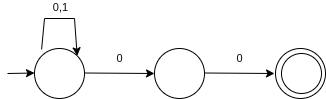
\includegraphics[width=0.6\textwidth,height=\textheight]{chapter03/imgs/endswith00.png}
\end{frame}

\begin{frame}[fragile]{Exemplo}
\protect\hypertarget{exemplo}{}
\begin{lstlisting}[language=Haskell]
endsWith00 :: NFA Int
endsWith00 = NFA 3 (Set.singleton 0)
    (\ s c -> case (s,c) of
        (0, '0') -> Set.fromList [0,1]
        (0, '1') -> Set.singleton 0
        (1, '0') -> Set.singleton 2
        _        -> Set.empty)
    (Set.singleton 2)
\end{lstlisting}
\end{frame}

\begin{frame}{Convers\~{a}o AFN -\textgreater{} AFD}
\protect\hypertarget{conversuxe3o-afn---afd}{}
\begin{itemize}
\tightlist
\item
  Seja \(M = (E, \Sigma, \delta, I, F)\) um AFN.
\item
  O AFD equivalente é:
\end{itemize}

\[M' = (\mathcal{P}(E),\, \Sigma,\, \delta',\, I,\, F')\]
\end{frame}

\begin{frame}{Convers\~{a}o AFN -\textgreater{} AFD}
\protect\hypertarget{conversuxe3o-afn---afd-1}{}
\begin{itemize}
\tightlist
\item
  \textbf{Estados} do AFD: subconjuntos de estados do AFN
\item
  \textbf{Estado inicial}: \(I\) (conjunto de estados iniciais do AFN)
\item
  \textbf{Estados finais}: \(F' = \{X \mid X \cap F \neq \emptyset\}\)
\item
  \textbf{Transi\c{c}\~{a}o}: \(\delta'(X, a) = \bigcup_{q \in X} \delta(q, a)\)
\end{itemize}
\end{frame}

\begin{frame}[fragile]{Implementa\c{c}\~{a}o}
\protect\hypertarget{implementauxe7uxe3o}{}
\begin{itemize}
\tightlist
\item
  O AFD resultante tem \textbf{estados do tipo
  \passthrough{\lstinline!Set a!}}
\item
  A transi\c{c}\~{a}o une os destinos de todos os estados do conjunto atual
\item
  Um conjunto é final se contém algum estado final do AFN
\end{itemize}
\end{frame}

\begin{frame}[fragile]{Implementa\c{c}\~{a}o}
\protect\hypertarget{implementauxe7uxe3o-1}{}
\begin{lstlisting}[language=Haskell]
subset :: Ord a => NFA a -> DFA (Set a)
subset m = DFA
  { start  = nfaStart m
  , delta  = \es c ->
      Set.unions (map (flip (nfaDelta m) c) (Set.elems es))
  , finals = \es ->
      not (disjoint es (nfaFinals m))
  }
\end{lstlisting}
\end{frame}

\hypertarget{expressuxf5es-regulares}{%
\section{Express\~{o}es Regulares}\label{expressuxf5es-regulares}}

\begin{frame}{Express\~{o}es Regulares}
\protect\hypertarget{expressuxf5es-regulares-1}{}
\[e \to \emptyset \mid \lambda \mid a \mid ee \mid e+e \mid e^*\]

\begin{itemize}
\tightlist
\item
  \(\emptyset\): conjunto vazio (nunca casa)
\item
  \(\lambda\): palavra vazia
\item
  \(a\): símbolo do alfabeto
\item
  \(ee\): concatena\c{c}\~{a}o
\item
  \(e+e\): uni\~{a}o (alternativa)
\item
  \(e^*\): fecho de Kleene (zero ou mais repeti\c{c}\~{o}es)
\end{itemize}
\end{frame}

\begin{frame}{Sem\^{a}ntica}
\protect\hypertarget{semuxe2ntica}{}
\[\begin{array}{lcl}
L(\emptyset) &=& \emptyset \\
L(\lambda) &=& \{\lambda\} \\
L(a) &=& \{a\} \\
L(e_1 e_2) &=& L(e_1)L(e_2) \\
L(e_1 + e_2) &=& L(e_1) \cup L(e_2) \\
L(e^*) &=& L(e)^*
\end{array}\]
\end{frame}

\begin{frame}[fragile]{Tipo Haskell para Express\~{o}es Regulares}
\protect\hypertarget{tipo-haskell-para-expressuxf5es-regulares}{}
\begin{lstlisting}[language=Haskell]
data Regex
  = Empty           -- ∅: conjunto vazio
  | Lambda          -- λ: palavra vazia
  | Chr Char        -- a: caractere específico
  | Regex :+: Regex -- e1 + e2: uni\~{a}o
  | Regex :@: Regex -- e1 e2: concatena\c{c}\~{a}o
  | Star Regex      -- e*: fecho de Kleene
\end{lstlisting}

\begin{itemize}
\tightlist
\item
  Operadores infixos (\passthrough{\lstinline!:+:!},
  \passthrough{\lstinline!:@:!}) refletem a nota\c{c}\~{a}o matemática
\item
  Construtores de dados representam diretamente a gramática
\end{itemize}
\end{frame}

\hypertarget{construuxe7uxe3o-de-thompson}{%
\section{Constru\c{c}\~{a}o de Thompson}\label{construuxe7uxe3o-de-thompson}}

\begin{frame}{A Ideia Central}
\protect\hypertarget{a-ideia-central}{}
\begin{itemize}
\tightlist
\item
  Converte ER em AFN por \textbf{recurs\~{a}o estrutural}
\item
  Para cada construtor da ER, há um AFN correspondente
\end{itemize}
\end{frame}

\begin{frame}{A Ideia Central}
\protect\hypertarget{a-ideia-central-1}{}
\begin{itemize}
\tightlist
\item
  AFNs parciais s\~{a}o \textbf{compostos} para formar o AFN final
\item
  Teorema: toda ER tem um AFN equivalente e vice-versa
\end{itemize}
\end{frame}

\begin{frame}{Caso Base: vazio}
\protect\hypertarget{caso-base-vazio}{}
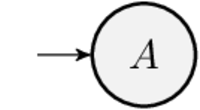
\includegraphics[width=0.3\textwidth,height=\textheight]{chapter03/imgs/image1.png}

\(e = \emptyset\): AFN sem estados, aceita a linguagem vazia
\end{frame}

\begin{frame}{Caso Base: lambda}
\protect\hypertarget{caso-base-lambda}{}

\includegraphics[width=0.3\textwidth,height=\textheight]{chapter03/imgs/image2.png}

\(e = \lambda\): um único estado que é simultaneamente inicial e final
\end{frame}

\begin{frame}{Caso Base: Símbolo}
\protect\hypertarget{caso-base-suxedmbolo}{}

\includegraphics[width=0.45\textwidth,height=\textheight]{chapter03/imgs/image3.png}

\(e = a\): dois estados, transi\c{c}\~{a}o sobre o símbolo \(a\)
\end{frame}

\begin{frame}{Caso Indutivo: Uni\~{a}o}
\protect\hypertarget{caso-indutivo-uniuxe3o}{}
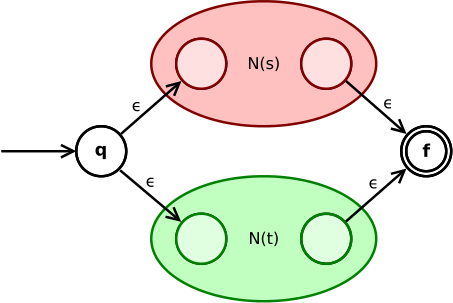
\includegraphics[width=0.6\textwidth,height=\textheight]{chapter03/imgs/image4.png}

\(e = s + t\): os AFNs \(N(s)\) e \(N(t)\) s\~{a}o colocados em
\textbf{paralelo}
\end{frame}

\begin{frame}{Caso Indutivo: Concatena\c{c}\~{a}o}
\protect\hypertarget{caso-indutivo-concatenauxe7uxe3o}{}
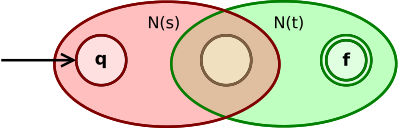
\includegraphics[width=0.65\textwidth,height=\textheight]{chapter03/imgs/image5.png}

\(e = s\,t\): os AFNs \(N(s)\) e \(N(t)\) s\~{a}o colocados em
\textbf{sequ\^{e}ncia}
\end{frame}

\begin{frame}{Caso Indutivo: Fecho de Kleene}
\protect\hypertarget{caso-indutivo-fecho-de-kleene}{}
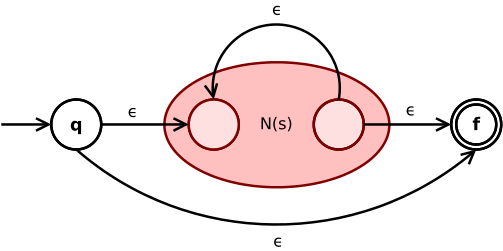
\includegraphics[width=0.55\textwidth,height=\textheight]{chapter03/imgs/image6.png}

\(e = s^*\): os estados finais de \(N(s)\) retornam aos estados iniciais
\end{frame}

\begin{frame}[fragile]{A Fun\c{c}\~{a}o \passthrough{\lstinline!thompson!} em
Haskell}
\protect\hypertarget{a-funuxe7uxe3o-thompson-em-haskell}{}
\begin{lstlisting}[language=Haskell]
thompson :: Regex -> NFA Int
thompson Empty = emptyNFA
thompson Lambda = lambdaNFA
thompson (Chr c) = chrNFA c
thompson (e1 :+: e2) = unionNFA (thompson e1) (thompson e2)
thompson (e1 :@: e2) = concatNFA (thompson e1) (thompson e2)
thompson (Star e1) = starNFA (thompson e1)
\end{lstlisting}
\end{frame}

\begin{frame}[fragile]{Pipeline Completo: ER → AFD}
\protect\hypertarget{pipeline-completo-er-afd}{}
\begin{lstlisting}[language=Haskell]
lexer :: [Regex] -> DFA (Set Int)
lexer = subset . foldr unionNFA emptyNFA . map thompson
\end{lstlisting}

\begin{enumerate}
\tightlist
\item
  \passthrough{\lstinline!map thompson!}: cada ER → AFN (via Thompson)
\item
  \passthrough{\lstinline!foldr unionNFA emptyNFA!}: combina todos os
  AFNs em um só
\item
  \passthrough{\lstinline!subset!}: converte o AFN combinado em um AFD
\end{enumerate}
\end{frame}

\hypertarget{crituxe9rio-do-maior-prefixo}{%
\section{Critério do Maior Prefixo}\label{crituxe9rio-do-maior-prefixo}}

\begin{frame}[fragile]{O Problema}
\protect\hypertarget{o-problema}{}
\begin{lstlisting}
if (x > 0) ift = x + 1;
\end{lstlisting}

\begin{itemize}
\tightlist
\item
  \passthrough{\lstinline!if!} é uma palavra reservada
\item
  \passthrough{\lstinline!ift!} é um identificador
\item
  O analisador precisa reconhecer o \textbf{maior prefixo} que forma um
  token válido
\item
  Sem esse critério: \passthrough{\lstinline!ift!} poderia ser lido como
  \passthrough{\lstinline!if!} + \passthrough{\lstinline!t!}
\end{itemize}
\end{frame}

\begin{frame}[fragile]{Por que o Maior Prefixo é Necessário?}
\protect\hypertarget{por-que-o-maior-prefixo-uxe9-necessuxe1rio}{}
\begin{itemize}
\tightlist
\item
  Garante que tokens compostos sejam reconhecidos \textbf{atomicamente}
\item
  Evita ambiguidades sem\^{a}nticas: \passthrough{\lstinline!>=!} n\~{a}o deve
  ser lido como \passthrough{\lstinline!>!} seguido de
  \passthrough{\lstinline!=!}
\end{itemize}
\end{frame}

\begin{frame}[fragile]{Por que o Maior Prefix é Necessário?}
\protect\hypertarget{por-que-o-maior-prefix-uxe9-necessuxe1rio}{}
\begin{itemize}
\tightlist
\item
  Padr\~{a}o universal em compiladores: \textbf{maximal munch}
\item
  Sem isso: \passthrough{\lstinline!integer!} poderia ser lido como
  \passthrough{\lstinline!int!} + \passthrough{\lstinline!eger!}
\end{itemize}
\end{frame}

\begin{frame}[fragile]{Implementa\c{c}\~{a}o}
\protect\hypertarget{implementauxe7uxe3o-2}{}
\begin{lstlisting}[language=Haskell]
longest :: DFA a -> String -> Maybe String
\end{lstlisting}

\begin{itemize}
\tightlist
\item
  Percorre a string mantendo o \textbf{último prefixo aceito} encontrado
\item
  O acumulador é uma tripla:
  \passthrough{\lstinline!(prefixo atual, melhor prefixo, estado atual)!}
\end{itemize}
\end{frame}

\begin{frame}[fragile]{Implementa\c{c}\~{a}o}
\protect\hypertarget{implementauxe7uxe3o-3}{}
\begin{itemize}
\tightlist
\item
  Retorna \passthrough{\lstinline!Nothing!} se nenhum prefixo é aceito
\item
  Retorna \passthrough{\lstinline!Just s!} com o maior prefixo aceito
\end{itemize}
\end{frame}

\begin{frame}[fragile]{Lógica da Fun\c{c}\~{a}o
\passthrough{\lstinline!longest!}}
\protect\hypertarget{luxf3gica-da-funuxe7uxe3o-longest}{}
\begin{lstlisting}[language=Haskell]
longest m = combine . foldl step (Just "", Nothing, start m)
  where
    step (Just pre, last, e) c
      | finals m (delta m e c) =
          (Just (c:pre), Just (c:pre), delta m e c)
      | otherwise =
          (Just (c:pre), last, delta m e c)
    step (Nothing, val, e) c =
          (Nothing, val, delta m e c)
    combine (_, val, _) = reverse <$> val
\end{lstlisting}
\end{frame}

\hypertarget{derivadas-de-expressuxf5es-regulares}{%
\section{Derivadas de Express\~{o}es
Regulares}\label{derivadas-de-expressuxf5es-regulares}}

\begin{frame}{Motiva\c{c}\~{a}o}
\protect\hypertarget{motivauxe7uxe3o-1}{}
\begin{itemize}
\tightlist
\item
  Thompson + subset pode ser computacionalmente custoso
\item
  Bibliotecas comuns (Java, Perl) usam \textbf{backtracking}: tempo
  exponencial
\end{itemize}
\end{frame}

\begin{frame}{Motiva\c{c}\~{a}o}
\protect\hypertarget{motivauxe7uxe3o-2}{}
\begin{itemize}
\tightlist
\item
  Derivadas de Brzozowski: abordagem alternativa eficiente
\item
  Permite construir AFD diretamente da ER, sem AFN intermediário
\end{itemize}
\end{frame}

\begin{frame}{A Ideia de Brzozowski}
\protect\hypertarget{a-ideia-de-brzozowski}{}
A \textbf{derivada} \(\partial(e, a)\) de uma ER \(e\) em rela\c{c}\~{a}o a um
símbolo \(a\) é a ER que aceita o \textbf{restante} da entrada após
consumir \(a\):

\[L(\partial(e, a)) = \{w \mid aw \in L(e)\}\]
\end{frame}

\begin{frame}[fragile]{Exemplos}
\protect\hypertarget{exemplos}{}
\begin{itemize}
\tightlist
\item
  Se \(e\) aceita \passthrough{\lstinline!"abc"!}, ent\~{a}o
  \(\partial(e, \text{'a'})\) aceita \passthrough{\lstinline!"bc"!}
\item
  Podemos construir o AFD computando derivadas sucessivas
\end{itemize}
\end{frame}

\begin{frame}{Anulabilidade}
\protect\hypertarget{anulabilidade}{}
Uma ER é \textbf{anulável} se \(\lambda \in L(e)\):

\[\begin{array}{lcl}
\nu(\emptyset) &=& \bot \\
\nu(\lambda) &=& \top \\
\nu(a) &=& \bot \\
\nu(e_1 e_2) &=& \nu(e_1) \land \nu(e_2) \\
\nu(e_1 + e_2) &=& \nu(e_1) \lor \nu(e_2) \\
\nu(e^*) &=& \top
\end{array}\]
\end{frame}

\begin{frame}[fragile]{Implementa\c{c}\~{a}o}
\protect\hypertarget{implementauxe7uxe3o-4}{}
\begin{lstlisting}[language=Haskell]
nullable :: Regex -> Bool
nullable Empty       = False
nullable Lambda      = True
nullable (Chr _)     = False
nullable (e1 :+: e2) = nullable e1 || nullable e2
nullable (e1 :@: e2) = nullable e1 && nullable e2
nullable (Star _)    = True
\end{lstlisting}
\end{frame}

\begin{frame}{Regras de Derivada}
\protect\hypertarget{regras-de-derivada}{}
\[\begin{array}{lcl}
\partial(\emptyset, a) &=& \emptyset \\
\partial(\lambda, a) &=& \emptyset \\
\partial(b, a) &=& \begin{cases} \lambda & \text{se } a = b \\ \emptyset & \text{c.c.} \end{cases} \\
\partial(e_1 + e_2, a) &=& \partial(e_1,a) + \partial(e_2,a) \\
\partial(e_1 e_2, a) &=& \begin{cases} \partial(e_1,a)\,e_2 + \partial(e_2,a) & \text{se } \nu(e_1) \\ \partial(e_1,a)\,e_2 & \text{c.c.} \end{cases} \\
\partial(e^*, a) &=& \partial(e,a)\,e^*
\end{array}\]
\end{frame}

\begin{frame}[fragile]{Implementa\c{c}\~{a}o}
\protect\hypertarget{implementauxe7uxe3o-5}{}
\begin{lstlisting}[language=Haskell]
deriv :: Char -> Regex -> Regex
deriv _ Empty  = Empty
deriv _ Lambda = Empty
deriv a (Chr b)
  | a == b    = Lambda
  | otherwise = Empty
deriv a (e1 :+: e2) = deriv a e1 .+. deriv a e2
deriv a (e1 :@: e2)
  | nullable e1 = deriv a e1 .@. e2 .+. deriv a e2
  | otherwise   = deriv a e1 .@. e2
deriv a (Star e1) = deriv a e1 .@. star e1
\end{lstlisting}
\end{frame}

\begin{frame}{Simplifica\c{c}\~{o}es Necessárias}
\protect\hypertarget{simplificauxe7uxf5es-necessuxe1rias}{}
Para que o conjunto de derivadas seja \textbf{finito}, aplicamos
simplifica\c{c}\~{o}es:

\[\begin{array}{ccc}
e_1 + \emptyset \equiv e_1 &
\emptyset + e_2 \equiv e_2 &
e_1 \emptyset \equiv \emptyset \\
\emptyset e_2 \equiv \emptyset &
e_1 \lambda \equiv e_1 &
\lambda e_2 \equiv e_2 \\
\lambda^* \equiv \lambda &
\emptyset^* \equiv \lambda &
(e^*)^* \equiv e^*
\end{array}\]
\end{frame}

\begin{frame}[fragile]{Simplifica\c{c}\~{o}es}
\protect\hypertarget{simplificauxe7uxf5es}{}
\begin{lstlisting}[language=Haskell]
(.+.) :: Regex -> Regex -> Regex
Empty .+. e' = e'
e .+. Empty  = e
e .+. e'     = e :+: e'
\end{lstlisting}
\end{frame}

\begin{frame}{AFD via Derivadas}
\protect\hypertarget{afd-via-derivadas}{}
\begin{itemize}
\tightlist
\item
  \textbf{Estados}: express\~{o}es regulares alcan\c{c}áveis por deriva\c{c}\~{a}o
\item
  \textbf{Transi\c{c}\~{a}o}: \(\delta(e, a) = \partial(e, a)\)
\item
  \textbf{Estados finais}: express\~{o}es anuláveis (aceitam \(\lambda\))
\item
  O conjunto de estados é sempre \textbf{finito} (com simplifica\c{c}\~{o}es)
\end{itemize}
\end{frame}

\begin{frame}[fragile]{AFD via Derivadas}
\protect\hypertarget{afd-via-derivadas-1}{}
\begin{lstlisting}[language=Haskell]
derivDFA :: Regex -> DFA Regex
derivDFA e = DFA
  { start  = simp e
  , delta  = \state c -> deriv c state
  , finals = nullable
  }
\end{lstlisting}
\end{frame}

\hypertarget{conclusuxe3o}{%
\section{Conclus\~{a}o}\label{conclusuxe3o}}

\begin{frame}{Conclus\~{a}o}
\protect\hypertarget{conclusuxe3o-1}{}
\begin{itemize}
\tightlist
\item
  \textbf{AFDs}: reconhecem linguagens regulares eficientemente
\item
  \textbf{AFNs}: facilitam a constru\c{c}\~{a}o por composi\c{c}\~{a}o (Thompson)
\end{itemize}
\end{frame}

\begin{frame}{Conclus\~{a}o}
\protect\hypertarget{conclusuxe3o-2}{}
\begin{itemize}
\tightlist
\item
  \textbf{Thompson}: converte ER em AFN por recurs\~{a}o estrutural
\item
  \textbf{Subset}: converte AFN em AFD equivalente
\end{itemize}
\end{frame}

\begin{frame}{Conclus\~{a}o}
\protect\hypertarget{conclusuxe3o-3}{}
\begin{itemize}
\tightlist
\item
  \textbf{Critério do maior prefixo}: resolve ambiguidades léxicas
\item
  \textbf{Derivadas de Brzozowski}: constroem AFD diretamente da ER
\end{itemize}
\end{frame}
